\subsection{Third Experience}

\subsubsection{Bulk TCP Transfer}

The three-way handshake is a way of establishing a connection between two PCs.
It makes sure that:

\begin{itemize}
    \item Sender is able to communicate with the receiver
    \item The receiver is able to listen
    \item The sender is able to listen to the receiver's response
\end{itemize}

After sending the text file, we analyzed the first three handshake packets.

\begin{figure}[htbp]
    \centering
    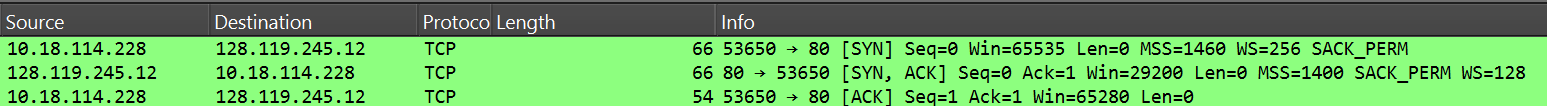
\includegraphics[width=1\linewidth]{img/third_experience/1.png}
    \caption{}\label{fig:3_1}
\end{figure}

After analyzing the contained headers, we can see that:

\begin{itemize}
    \item The first packet is a SYN (synchronize) packet sent from the sender to the
          receiver. Its sequence value is 0.
    \item Shortly after, the receiver responds with a SYN-ACK (synchronize-acknowledge)
          packet. The ACK value was set to 1, which means that the receiver acknowledged
          the sender's sync request.
    \item Finally, the sender responds with an ACK package and sequence value set to 1.
          This means that the connection was established, and the sequence step (stage)
          is now 1 (data transfer enabled).
\end{itemize}

After this short analysis, we can see that the ACK value is set to 1 after the
receiver \textbf{ACKnowledges} the sender's request. It's a way confirming the
connection request.

The ports used for communication were:

\begin{itemize}
    \item Sender SYN:\@ 53650 to 80
    \item Receiver ACK:\@ 80 to 53650
    \item Sender ACK:\@ 53650 to 80
\end{itemize}

Disabling capture of HTTP packets in Wireshark stops them from showing up in
the Wireshark dashboard.

Clicking on any TCP packet and following the stream shows the entire
communication sequence with the sent and received packets in a readable format.
On the bottom left, we can see that 18 packets were needed to send the entirety
of the text content.

The sequence number of a TCP packet is a number that identifies the order of
the packet being sent. It's sent according to the previous' packet sequence
number length.

\subsubsection{Captured Trace}
